\documentclass{article}
\usepackage[utf8]{inputenc}
\usepackage[utf8]{inputenc}
\usepackage{epigraph}
\usepackage{xcolor}
\usepackage{graphicx}
\usepackage{anyfontsize}
\usepackage{fancyhdr}
\pagestyle{fancy}
\usepackage{lastpage}
\usepackage{graphicx}
\usepackage{fancyhdr}
\usepackage{verbatim}
\pagestyle{fancy}
\usepackage{lastpage}
\renewcommand\headrulewidth{1.4pt}
\fancyhead[R]{Computer Studies}
\renewcommand\footrulewidth{1.4pt}
\fancyfoot[C]{\thepage}
\fancyfoot[R]{\today}
\usepackage[UKenglish,USenglish]{babel}
\title{Computer Studies}
\author{bijan.veyssi-galmiche }
\date{March 2020}

\begin{document}
\maketitle
\newpage
\section{Gschem}
I learnt to use gschem, it was pretty easy since it is very intuitive. You will find what I did on it beneath.
\newline
\begin{center}
\includegraphics[angle=0, width=12cm]{01.png}
\newline
\textit{Here is the scheme obtained after printing}
\end{center}{}
\section{Ngspice}
\verbatiminput{01.net}
\textit{Here is .net file obtained}
\section{Results}
\begin{verbatim}
ngspice 1 -> source 01.net

Circuit: * spice netlister for gnetlist

ngspice 1 -> tran 5 1
Doing analysis at TEMP = 27.000000 and TNOM = 27.000000


Initial Transient Solution
--------------------------

Node                                   Voltage
----                                   -------
2                                      28.1212
1                                           32
v1#branch                            -0.242424



No. of Data Rows : 59
ngspice 1 -> plot "1"
ngspice 1 -> plot "2"
\end{verbatim}
\begin{center}
\textbf{Here is the result of plot "1"}
\includegraphics[angle=0, width=12cm]{011.eps}
\textbf{And here is the result of plot "2"}
\includegraphics[angle=0, width=12cm]{012.eps}
\end{center}{}
\end{document}

